\section{Introduction}
\label{sec:intro}

\paragraph{Motivation}
Programming systems that interact with physical processes are central in  robotics, manufacturing, IoT, and other cyberphysical systems. Typical domain specific languages (DSL) for these systems are platform specific and they combine  low-level sensing, communication, and control tasks with the application-level logic~\cite{nordmann2014robotics}. This  tight-coupling of applications with platform-specific details can hinder development, modularity, portability, code reuse, and testing. 

This need for raising the level of abstraction and separating the \emph{platform-independent} from the \emph{platform-dependent} concerns motivates our work. For example, consider an application for distributed package delivery with mobile robots in a building. The higher-level coordination has to deal with assigning robots to visit way-points in different rooms, load-balancing, and handling failures.  For all of the reasons mentioned above, these coordination tasks {\em should be\/} separated from the  steering control of the individual vehicles, indoor positioning, and message-level communication protocols tied to the specific hardware platforms. 

Current programming languages do not natively support such abstractions for programming distributed cyberphysical systems.  The developer will have to keep track of communication between different sensors, actuators, and program variables. The {\em robotic operating system (ROS)}~\cite{rosbridge_suite,ros} does provide useful libraries and  publish-subscribe messaging standards, but these are not integrated in a programming abstraction. Similarly, coordination across multiple robots has to be built from the ground up using message passing threads. In order to simulate and test the application, one has to create different threads or instances for the developed code corresponding to different agents, and on top of that, the agent programs have to be harnessed in a physical world simulator with proper sensor and actuator models. In order to analyze correctness, one has to first define the semantics of the system. This  is again challenging  as  distributed cyber-physical systems have concurrency and data flows in multiple time-scales. 
%A further source of concern is the gap between the system model with iand the executable code that is actually . 

An ongoing, multi-year, project at our lab aims to address some of these challenges by designing, developing, and evaluating a programming system for distributed robotics. \footnote{Information about this project and the links to downloadable software will be made available to the reviewers upon request. We omit the information here for the sake of maintaining anonymity.} In this paper, we present the design and the implementation of the  {\em $\lgname$ language} and the supporting software tools, which form the  core of this programming system.


%
%\begin{figure}[h!]
%\centering
%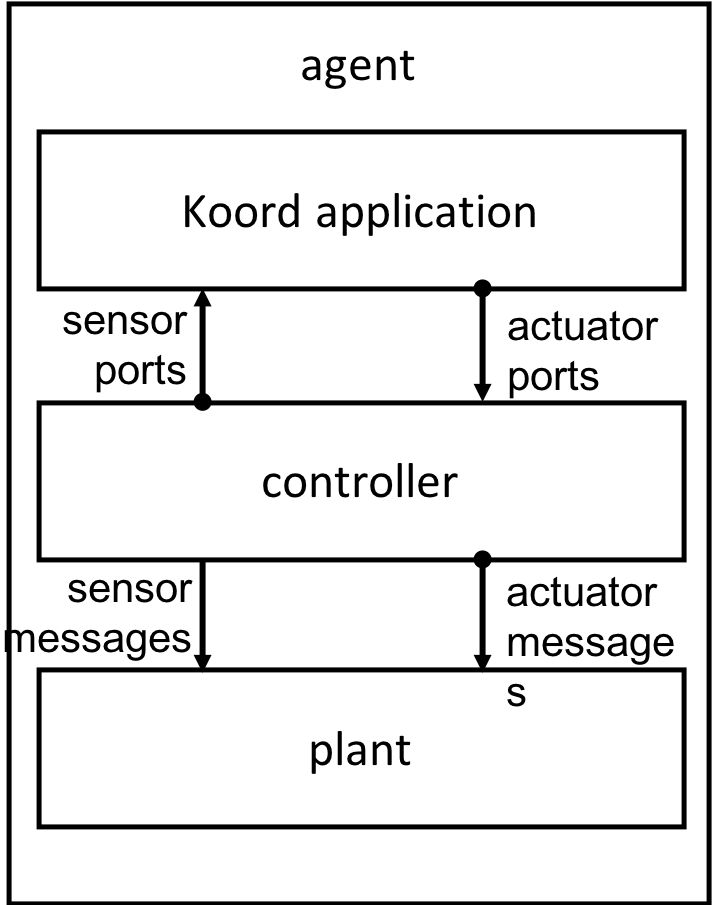
\includegraphics[width=0.48\textwidth]{figs/arch.png}
%\caption{\small CyPhyHouse framework. Major tools shown in blue.}
%\label{fig:arch}
%\end{figure}
%
\subsection{Contributions}
\subsubsection{Design and implementation of $\lgname$ language}
{\em We present a clean-slate design and implementation of an event-driven programming language, for distributed cyber-physical systems, namely $\lgname$.} 
%
$\lgname$ combines distributed shared memory abstraction for coordination across agents and a synchronous model of communication with the physical environment through sensors and actuators, all packed in a familiar precondition-effect style language.
%

Consider a simple line-formation program in which a set of $N$ robots form a equi-spaced line starting from arbitrary positions. The elementary algorithm is for each robot $i$ to repeatedly move towards the midpoint of the line joining the positions of $i-1$ and $i+1$. The extremal robots with ids $0$ and $N-1$ stay fixed. This is a archetypal protocol for synchronization, pattern formation, and consensus~\cite{Tsitsiklis:1986,Blondel,Magnusbook2010,Fax} in distributed robotics.
%
% \belowcaptionskip=-10pt
\begin{lstlisting}[label=lineform,caption=Lineform $\lgname$ program]
   using Motion:
      sensors pos psn
      actuators target
   allread: pos x $\label{lineformp}$
   TargetUpdate:
      pre True
      eff if not(pid == $\NMAX$ - 1 or pid == 0):
         Motion.target = mid(<x[pid+1],x[pid-1]>)
         x[pid] = Motion.psn
\end{lstlisting}

The above $10$ line  $\lgname$ program implements this line formation algorithm and can be simulated or deployed (see Figure~\ref{fig:shapeformplots1}). Among these $10$ lines of code, lines 1-5 import the {\em controller module\/} called {\em Motion\/} that enables this program to access the sensor port with the agent's position $(\mathit{psn})$ and the actuator port $(\mathit{target})$. An implementation of  a {\em controller module\/} has platform-specific path planners and low-level controllers for moving specific types of robots in the physical world. {\em Thus, with different implementations of the {\em Motion\/} interface the $\mathit{Lineform}$ $\lgname$  program can be ported to different platforms\/}. 

Another powerful feature of $\lgname$ used in the $\mathit{Lineform}$ program is the single-write multi-reader ({\bf allread}) shared array $x$, in which component $x[i]$ records the position of the $i^{th}$ robot in each round.  Shared variables allow the participating agents programs to coordinate without exposing the programmer to explicit message passing channels, buffers, and threads. This makes $\lgname$ programs succinct, readable, and often, as in the  above example, remarkably close to the textbook version of the algorithm. The $\lgname$ runtime system (discussed in more detail in Section~\ref{sec:software}) implements the propagation of  the shared variable write over messages. The formalization of the resulting semantics is discussed in Section~\ref{sec:K}.

%
The one and only event in the $\mathit{Lineform}$ program is $\mathit{TargetUpdate}$ (lines 5-9): it updates the target position of the agent  to be the midpoint of its neighbors.  Figure~\ref{fig:shapeformplots} shows the result of simulating a slightly modified version of $\mathit{Lineform}$ on the $\lgname$ simulator with $25$ robots forming a 3D-shape. The $\lgname$ compiler can also generate executables that can be deployed on several mobile robotic hardware platforms such as F1/10 cars~\cite{f1-10}, drones~\cite{}, and Roombas. We mention these capabilities briefly in Section~\ref{sec:intro:hardwaretc}, however, the platform-specific details for will be presented in a future article. 

%\renewcommand{\lstinputlisting}[1][]{\oldlstinputlisting[frame=lines,#1]}
 
%\begin{figure}[ht!]
%	\label{fig:lineform}
%	\noindent
%	\begin{center}
%		\scriptsize
%		\two{0.4}{0.6}
%		{\lstinputlisting[language=xyzNums,frame=lines]{code/lineform.tex}}
%	\par        
%	\end{center}
%	\caption{\small $\lgname$ program for line formation ({\em Left}) and its mathematical counterpart in robotics and control textbooks ({\em Right}).}
%\end{figure}

%The shared \emph{allread} variable $p$ (Line\ref{lineformp}) is used by the agents to communicate their position to the other robots. The function \emph{midpoint} is a part of the library functions provided for the data type \emph{pos}; where $$\mathit{midpoint}(p_1,p_2,\ldots,p_n) = pos(\frac{\Sigma_n p_i.x}{n},\frac{\Sigma_n p_i.y}{n},\frac{\Sigma_n p_i.z}{n}) $$.
%

%We have implemented a compiler for $\lgname$ that generates executable Python programs that can be either simulated in a discrete event simulator (discussed below) or 

\subsubsection{\K semantics for $\lgname$}
% motivation
Implementation of programming languages usually have many bugs. One common source of bugs is the gap between the formal semantics of the language and the its implementation as embodied in a compiler. The \K framework~\cite{Kf} closes this gap by allowing the specification of {\em  formal executable semantics of any programming language} in terms of  rewrite rules. These rewrite rules define how each and every possible statement in the  language changes, possibly nondeterministically, the state of the machine executing the program. 
%
\K  provided the most-complete-to-date formal definition of the C language~\cite{KC}. As the \K semantics is executable, \sayan{this semantics was tested against the GCC torture test suite and successfully passed 99.2\% of 776 test programs~\cite{chuckythesis}. What does this mean?} More recently, \K  was used to provide a formal semantics of x86-64~\cite{rusuadvepaper} and its formal analysis capabilities were used to verify the Ethereum Virtual Machine (EVM) bytecode. 


%\K  using computations over states or configurations, and rewrite rules for said configurations. \K has several additional features including non deterministic execution, underspecification and explicit read-only and write only specifications for rewrite rules which makes \K suitable for defining concurrent and control intensive languages. 
{\em In order to close the above-mentioned gap, we have developed the complete executable formal semantics of $\lgname$ in \K.} 
\sayan{This is the first formalization of a language for distributed systems in \K.} 
Some of the main challenges presented during this were designing the shared memory semantics keeping in mind that it would be eventually implemented through message passing, and adding the controller behaviors with path-planners to the back-end of \K to specify rewrite rules for them, as the $\lgname$ language itself lets the user use predefined controller modules. \fTBD{THIS STATEMENT IS NOT CLEAR, HOW DO I PHRASE THIS?}

Our intent with this language is to provide a way of programming \emph{safe} distributed cyber-physical applications. Our \K implementation of $\lgname$ enables us to execute \emph{semantically accurate} programs automatically, so we can to design test suites for any implementation of the language semantics. To support formal analysis in case of non-specific initial states, we also implemented an interval arithmetic in \K, and support execution of $\lgname$ programs where the initial values of variables are provided in intervals. We implemented a explicit state bounded-model-checking verification tool on top of the \K semantics to provide this additional feature. 


\subsubsection{Simulator and applications}

We developed a simulator \reffig{simulator} for $\lgname$ applications within the CyPhyHouse framework. 

The major challenges involved in designing a simulator were to create a simulation engine that exactly simulates the behavior expected on hardware deployment. To that end, the simulator uses motion automata, which can be provided any programmable dynamics to simulate the robot dynamics. The simulated sensed data can also be also provided realistic noises and dynamics to mimic actual system dynamics. The communication protocols to propagate shared memory messages between agents are also a part of the simulator communication module. The time between two computational steps (or discrete event loop iterations) is used to propagate messages to implement shared memory as in the actual hardware stack.

The simulator enables the user to test their discrete event loop with simple motion models to test and debug the application program logic without incurring the cost of hardware deployment in case of buggy programs. The simulator also serves as a visualization tool as it can be used to plot the behavior of any program variables, or controller variables. For instance, we implemented a robot \emph{formation} app in $\lgname$, where several robots form a shape in which they are evenly distributed.


\begin{figure}[h!]
\begin{minipage}{0.5\textwidth}
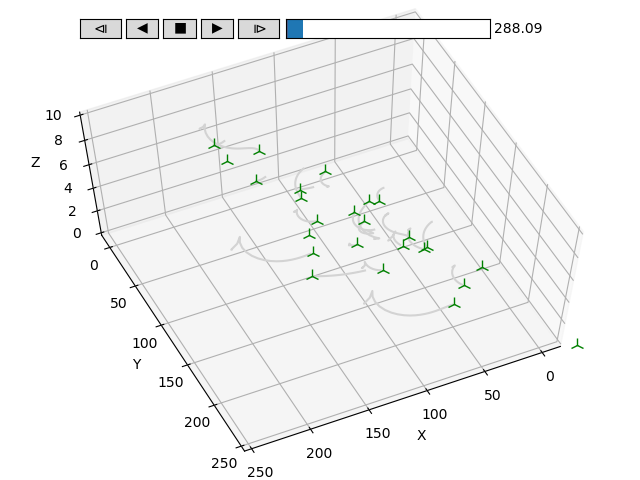
\includegraphics[width=.5\textwidth]{figs/formation1.png}\hfill
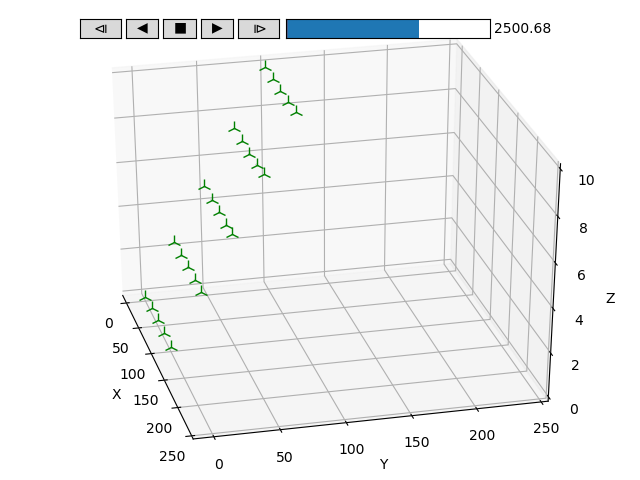
\includegraphics[width=.5\textwidth]{figs/formation5.png}\hfill%
%\includegraphics[width=.3\textwidth]{figs/Platooning_2.png}}\hfill%
\end{minipage}%
\caption{$x$ vs $y$ vs $z$ plots for a robot formation application. The grey trails represent the positions of the agents in the last 150 time steps.}
\label{fig:shapeformplots1}
\end{figure}


\subsubsection{Other by-products}


Design and development of the CyPhyHouse open source software system. This includes a discrete event simulator for distributed robotic systems, the application launcher, the run-time logging and monitoring system, and an integrated indoor positioning system. All of these software tools are integrated with our new robot programming language called $\lgname$ and its compiler. 

 First demonstration of the feasibility of end-to-end high-level application development and deployment on a distributed, heterogeneous, platform involving quadcopters and ground vehicles. 

 Demonstration of the feasibility of system-level verification of applications written in $\lgname$. 

Design and development of the $\lgname$ programming language and the supporting $\mathbb{K}$-based~\cite{Kpaper} verification tool \kbmc\, are discussed here for the sake of completeness; those details will appear elsewhere~\cite{koordreport}.

%Design and development of the Koord programming language and the supporting verification tool KoordBMC~\cite{koordreport}--- significant, related but separate efforts---are not contributions of the current paper; we discuss their usage for the sake of completeness. 
% completely describing the framework. 
% the Demonstration of an example application development using CyPhyHouse tools and deployment on a physical system using multiple quadcopters.
%Non-contributions: Spell these out  to avoid misdirected criticisms and conflict with overlapping publications.
%\begin{itemize} 
%\item Language design
%\item Verification tools.
%\item Low-level controller design for vehicles.
%\end{itemize} 

%\begin{figure}[h!]
%\centering
%\includegraphics[width=0.45\textwidth]{figs/exp_traces.png}
%\caption{\small Experimental run in our testbed. The traces show the path of each robot for the last $2$ seconds. }
%\label{fig:exp_traces}
%\end{figure}


\footnote{\href{https://cyphyhouse.github.io/index.html}{https://cyphyhouse.github.io}}: an open source software framework for programming, rapid deployment, and testing of distributed robotics applications. 
\sayan{The high-level $\lgname$ language enables users to write succinct distributed coordination applications without getting bogged down by messaging and thread management issues (See Examples in \reffig{lineform} and \reffig{taskapp}).}
Using the CyPhyHouse framework around $\lgname$, a user can code, compile, launch, and run applications in a highly-automated fashion (\reffig{arch}). 
\sayan{The framework has been built over three years and has more than 100k lines of source code.}


    - problems in the space of (distributed) CPS, robotics, automation .
    - Coordination and Control issues. 
    - why we need something like Koord /why something like koord helps computer scientists (non roboticists) work with robotics. 
    - what is koord and how Koord specifically accommodates users
    - how we built koord. 
    - what is this paper
    - Related work
    
    \section{Related work}
    \label{sec:related}
    \sayan{Modern programming languages like C\# and Swift, and   compiler infrastructures like LLVM~\cite{llvm} have revolutionized the application development ecosystem in mobile computing.
%\paragraph*{D.} 
Inspired by these successes, there is a surge of interest in open and portable languages that raise the level of abstraction~\cite{Buzzlanguage,Bohrer:2018:VVC:3192366.3192406,reactlang,williams2003model} (For an earlier survey of Domain Specific Programming Languages (DSLs) for robotic systems see~\cite{Nordmann2014}. Most of these older languages are proprietary or generate executable files that are tied to specific platforms)}. 
%
Buzz~\cite{Buzzlanguage} and React~\cite{reactlang} fall in this category as does our language $\lgname$. 
The Live Robot Programming language~\cite{campusanofabry:lrp2016} not only provides a higher-level programming abstraction in terms of nested state machines, but also allows the program to be changed while running, hence reducing the feedback loop across writing, compiling, and testing of robot programs. 
%The goals of React language for robotics aligns with our goals~\cite{react-lang}
Buzz currently does not  connect with  verification tools, and the verification approach implemented with React uses precise models of the environment and performs model checking using dReal~\cite{Gao2013}. 
In contrast, our environment implementations allow for imprecise models, with a verification approach using sensitivity analysis~\cite{DryVR2017}.
%Our approach is also similar in spirit to the Reactive Model-based Programming Language (RMPL)
%~\cite{williams2003model}.
%
%There is been more recent development of domain specific languages for general cyber-physical systems (CPS)~\cite{pradhan2015chariot}. The main challenge addressed in this line of work is in supporting reconfiguration of complex, heterogeneous software components, for handling failures. 
%
%There has also been work on programming abstractions for coordinating CPS~\cite{distCPSSri,Bundle}. 
%A group-based abstraction that facilitates dynamic creation of logical collections of sensors and actuators is presented in~\cite{Bundle}. 
%
%
%%React reactive robot programming language~\cite{DogmusEP15}.
%% 
The Robotarium project provides remote end-to-end access to a  multi-robot research facility, but not languages and development tools~\cite{robotarium}. 
The  VeriPhy project~\cite{Bohrer:2018:VVC:3192366.3192406} shares a similar goal to CyPhyHouse; however, instead of a programming language, the starting point is differential dynamic logic~\cite{Bohrer:2017:FVD:3018610.3018616},  and there are significant differences  in the underlying verification engines used (KeYmaera X, HOL instead of K, Z3, DryVR).
%

``Correct-by-construction'' synthesis from high-level temporal logic specifications has been applied to mobile robotic systems (see, for example~\cite{kress2009temporal,kloetzer2008fully,wongpiromsarn2010receding,wongpiromsarn2011tulip,ulusoy2013optimality}).
% Many of these approaches have been applied to mobile robotic systems. 
\sayan{Our point of view on automating robot programming is different in that we expect that the programmer's creativity and efforts will be necessary well beyond writing high-level specs in solving distributed robotics problems; consequently only the tedious and standard steps in coordination and control are automated using the $\lgname$ compiler.}

%. A
%correct-by-construction synthesis algorithm takes as input a high-level requirement (for example, ``from room A to B and see if you find a chair'') to generate robot programs for accomplishing
%this task. In our approach, 

%\paragraph*{Languages for distributed shared memory systems}
%
Programming systems using the  shared memory paradigm have been developed for several distributed computing systems~\cite{dsm1991,Adve96sharedmemory,Azure,Cassandra,Dynamo}.
Specifically, P~\cite{Planguage}  and PSync~\cite{PSyncLanguage} are DSLs for  asynchronous partially  distributed systems, but cyber-physical interactions are not supported. 
%DSM has also been proposed as a programming model in the context of wireless networks~\cite{hcs,rs}. 
%These  programming models are defined mathematically in terms of state machines or in terms of APIs, and are  typically not embodied in a programming language with carefully designed syntax and semantics to enforce the models. 
$\lgname$  provides a distributed shared variable abstraction for coordinating multiple agents. 
%\sayan{This enables users to write succinct, textbook-like programs without struggling with messy code for message handling and thread management}. 
The consistency semantics implemented here are that the writes to shared variables are propagated to all the agents, and become visible to other agents reading the variable after one round ($\delta$ time units).
In the fault-free synchronous model considered here a gossip algorithm-based is used to implement this semantics in the $\lgname$ runtime system. 
% The framework of~\cite{Hotline_CPS_srivastava} supports shared memory over multi-hop wireless networks, with a consistency model analogous to {\em release} consistency.  
%

%
%\paragraph*{Uncertainty and Robotics Abstractions}
%$\lambda_O$~\cite{park2005probabilistic} is a probabilistic programming language in which sampling methods are used to specify probability distributions, while expressing and reasoning about these methods formally. It finds application in robot localization and mapping. In the same vein, $\mathit{Uncertain}\langle T\rangle$~\cite{bornholt2014uncertain} provides a programming language abstraction for uncertain data. It is a departure from previous probabilistic programming languages in the wide range of developers it serves, as opposed to being accessible only by experts. The language provides abstractions and semantics for uncertain data, like sensed information about location, temperature, etc. While $\lgname$ does not currently perform reasoning involving uncertainty in sensor readings or agent localization currently, these are realistic concerns that can be explored by exploiting the extensibility of the $\lgname$ semantics implemented in \K. While these languages provide semantics for uncertainity in robot abstractions and sensing issues, they do not provide distributed application design capabilities. 
%\sayan{I did not find much about this. Formal verification of mobile robot protocols: the DVE language, which is the input format of the model-checkers DiVinE and ITS tools, and formally prove the equivalence of the two models.}
%\item  
%Buzz, a novel programming language for heterogeneous robot 
%swarms. Buzz advocates a compositional approach, offering primitives to define swarm 
%behaviors both from the perspective of the single robot and of the overall swarm. 
%
%\item 

%Voltron programming system to explore the concept of team-level programming in active sensing applications. Voltron offers programming constructs to create the illusion of a simple sequential execution model while still maximizing opportunities to dynamically re-task the drones as needed. We implement Voltron by targeting a popular aerial drone platform, and evaluate the resulting system using a combination of real deployments, user studies, and emulation. Our results indicate that Voltron enables simpler code and produces marginal overhead in terms of CPU, memory, and network utilization. In addition, it greatly facilitates implementing correct and complete collaborative drone applications, compared to existing drone programming systems. (?) 
%\end{enumerate}

